\documentclass[11pt]{article}
\usepackage[includeheadfoot, top=1.0in, bottom=1.0in, hmargin=1.0in]{geometry}
\usepackage[utf8]{inputenc}
\usepackage{fancyhdr}
\usepackage{url}
\pagestyle{fancy}
\usepackage{setspace}
\usepackage{tabularx}
\usepackage{graphicx}
\usepackage{caption}
\usepackage{subcaption}
\usepackage{hyperref}
\usepackage{multicol}


\lhead{Astronomy Lab II}
\rhead{Spring 2023}
\lfoot{Golant}
\rfoot{Tues 7-10pm}
\cfoot{\thepage}

\begin{document}

\begin{center}
\huge{Lab 3: Spectroscopy}\\ \medskip \Large{February 07, 2023}
\end{center}

%%%%%%%%%%%%%%%%%%%%%%% INTRO %%%%%%%%%%%%%%%%%%%%%%%
\section{Introduction: The Rainbow Connection}
The earliest appearance of the term ``astrophysics'' in the literature comes from an 1865 series of lectures on \emph{\textbf{spectroscopy}} by Johann Z\"{o}lner. While spectroscopy had been a well-established technique in chemistry and laboratory physics, its application to astronomy was novel -- for the first time, the physics of the lab was being applied to the objects of the heavens. 

Spectroscopy is the study of the light that objects emit or absorb. Last lab, we saw that the Universe is filled with a myriad flavors of light, spanning orders of magnitude in wavelength. Spectroscopy hones in on a specific object and holistically studies the range of wavelengths emitted or absorbed by that object -- the set of light emitted or absorbed by an object is called the object's \emph{spectrum}. An object's spectrum can provide a remarkable amount of information; the spectrum tells us about the chemical makeup of the object, the motion and speed of the object, the temperature of the object, the distance to the object (in certain contexts), and much more. Thus, spectroscopy is an extremely popular technique for studying planets, stars, galaxies, and the vast zoo of objects populating our Universe.


Recall that last week we briefly examined how different wavelengths of light behave when passed through a prism (if you need a refresher, here's the applet we used \url{https://javalab.org/en/electromagnetic_waves_around_of_visible_rays_en/}). In the last lab, I posed the question: ``If we were to shine \emph{starlight} through a prism, what could the resulting light pattern tell us about the star?'' Today, we will work to answer this question.

%%%%%%%%%%%%%%%%%%%%%%% BLACKBODY %%%%%%%%%%%%%%%%%%%%%%%
\section{Blackbody Radiation}

Before we dive into the spectra of real objects, we'll consider the simplified, idealized model of a \emph{blackbody}. A blackbody is an object that perfectly \emph{absorbs} all wavelengths of light, with no reflection. If a blackbody is heated to a temperature above absolute zero, it will also \emph{emit} light at all wavelengths. \textbf{Answer the following questions in your lab write-up}:
\begin{enumerate}
    \item Consider the processes of \emph{emission}, \emph{absorption}, and \emph{reflection} (or \emph{``scattering''}) of light.
    \begin{enumerate}
        \item Define these three terms in your own words (though you may use online resources for information).

        \item What determines the perceived color of an object?

        \item Why don't all objects appear white?

        \item Why do you think a blackbody is called a ``blackbody"?
    \end{enumerate} 
    
\end{enumerate}

%The Planck Spectrum and Wien's Law
Plotting the intensity (or brightness) of light at each wavelength emitted by a blackbody yields the \emph{blackbody spectrum}. Although blackbody spectra are smooth and idealized, it's often fairly accurate to approximate stars and other astronomical objects as blackbodies. We'll explore the ways in which real spectra deviate from blackbody spectra in later sections.

\bigskip

For now, though, let's examine the blackbody spectrum hands-on. Navigate to \url{https://phet.colorado.edu/sims/html/blackbody-spectrum/latest/blackbody-spectrum_en.html}. The plot to the left of the screen shows a blackbody spectrum, with spectral power density (just a fancy way of quantifying the amount of light emitted) on the vertical axis (in units of Megawatts per square meter per micrometer) and wavelength on the horizontal axis (in units of micrometers). To the right of the screen is a thermometer showing the temperature of the blackbody. Make sure to check the boxes for ``Graph Values" and ``Labels" in the box to the upper right; after turning on these features, you should see a pair of yellow numbers labeling the \emph{peak} of the blackbody curve. You can click and drag the slider on the thermometer to change the temperature of the object. If you need to adjust the size of your graph to see the full curve, you can use the zoom buttons (the magnifying glasses) to the upper left and bottom right of the plot.

\bigskip
\textbf{Make a table with three columns: 1) temperature (in units of K); 2) the wavelength (in units of $\rm \mu m$) corresponding to the peak of the spectrum (i.e., the value labeled by the yellow number on the horizontal axis); and 3) the \emph{reciprocal} of the peak wavelength (in units of $\rm 1/\mu m$). Record the following in your lab write-up}: 
\begin{enumerate}
    \setcounter{enumi}{1}
    
    \item Test at least 5 different temperatures across the full range of the thermometer and fill out the columns in your table. Report your numbers using \emph{two} significant figures.
    \item Qualitatively, what do you notice about the relationship between temperature and peak wavelength? Do temperature and peak wavelength vary directly with one another, or do they vary inversely?
    \item Make a plot of your data with the \emph{reciprocal} of the peak wavelength on the vertical axis and the temperature on the horizontal axis. Make sure to label your axes with the correct units! What do you notice about this plot? 
    \item Make a new column in your table and calculate the value of the peak wavelength \emph{multiplied} by the temperature (using two significant figures). What do you notice about these values? 
\end{enumerate}

\medskip \noindent
Congratulations! You've just derived \textit{Wien's law}, a very useful equation in astronomy. Because the product of the peak wavelength and the temperature is always the same number, we can derive the surface temperature of an object (like a star) by measuring the wavelength at which the object emits most of its light. In math, Wien's law reads
\begin{equation}
    \lambda_{\rm peak} \times T = \left(2.9 \times 10^3 \right) \, {\rm \mu m \, K},
\end{equation}
where $\lambda_{\rm peak}$ is the peak wavelength (in $\rm \mu m$) and $T$ is the temperature (in K). Let's use Wien's law to answer a few questions. \textbf{Record your answers in your lab write-up}.
\begin{enumerate}
    \setcounter{enumi}{5}
    
    \item Are redder objects hotter or cooler than bluer objects? (note that this applies to both the flames on our kitchen stoves and to the stars illuminating the night sky)
    
    \item The surface temperature of the Sun is around $5780 \, {\rm K}$. 
    \begin{enumerate}
        \item At which wavelength does the Sun emit most of its light (give your answer in $\rm \mu m$ to two sig figs)?
        \item What color of light does the Sun emit the most?
    \end{enumerate} 
    
    \item The \emph{cosmic microwave background} (CMB) is the oldest perceptible light in the Universe. Since the CMB permeates the entirety of outer space, the temperature of the CMB is often referred to as simply the temperature of the Universe. The CMB forms a remarkably perfect blackbody spectrum, with a peak wavelength around $1.06 \, {\rm mm}$ (see Figure \ref{fig:CMB}). 
    \begin{enumerate}
        \item What is the temperature of the Universe (in K, to two sig figs)? Be careful of units!
        
        \item Is this temperature hotter or colder than you were expecting? (for reference, $\rm 1 K = -272 \, ^\circ C = -458 \, ^\circ F$)
        
        \item Why is ``cosmic \emph{microwave} background'' an appropriate name for this light? 
    \end{enumerate}
\end{enumerate}

\begin{figure}[h!]
    \centering
    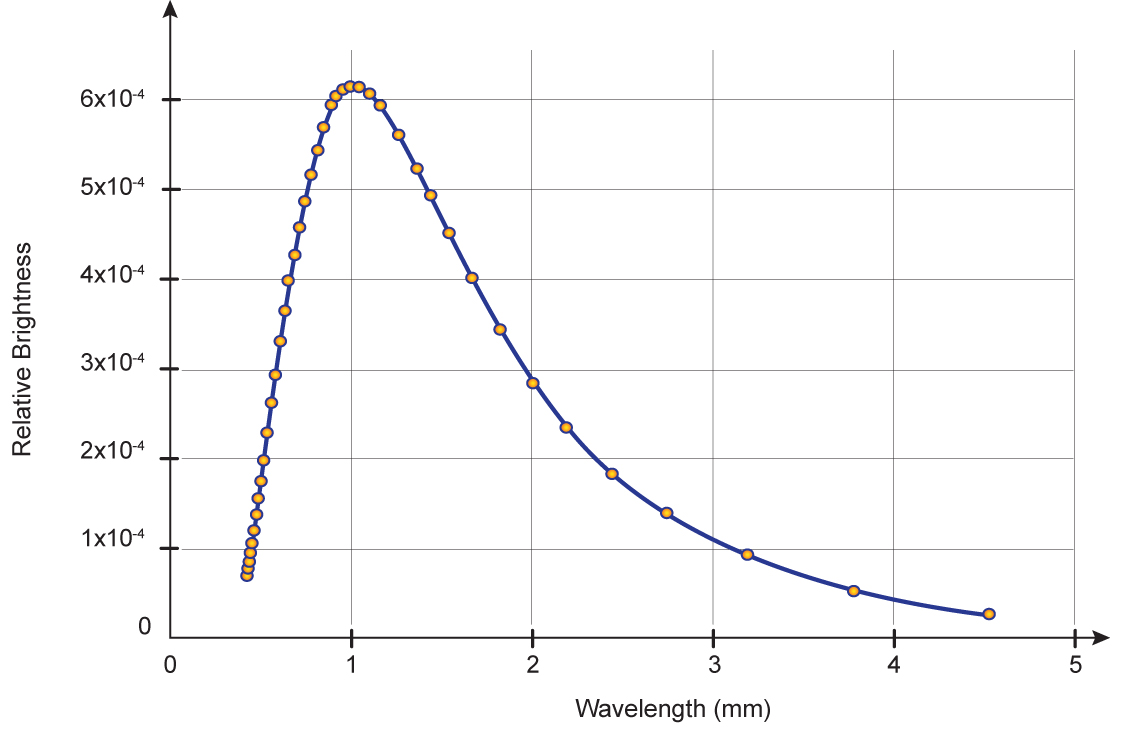
\includegraphics[width=0.7\textwidth]{Images/CMB.jpg}
    \caption{Spectrum of the cosmic microwave background (CMB).}
    \label{fig:CMB}
\end{figure}


%%%%%%%%%%%%%%%%%%%%%%% ELEMENTS %%%%%%%%%%%%%%%%%%%%%%%
\section{Fingerprints of the Elements}

The blackbody spectrum is a perfectly smooth spectrum. In reality, however, objects (like stars and galaxies) possess many ``features'' -- or \emph{lines} -- in their spectra that can tell us much more than just the temperature of the object. Let's explore some real spectra now.

Figure \ref{fig:spec} shows examples of two different real spectra. On the horizontal axis, we have the wavelength of light (as was also the case in the blackbody spectrum); in general, spectra can cover wavelengths of light spanning the entire electromagnetic spectrum. On the vertical axis, we have \textit{flux}, another measure for how much light is being emitted and detected (in particular, flux measures the amount of light passing through a given area in a given amount of time).

\bigskip

\begin{figure}[h!]
    \centering
    \begin{subfigure}[b]{0.75\textwidth}
        \centering
        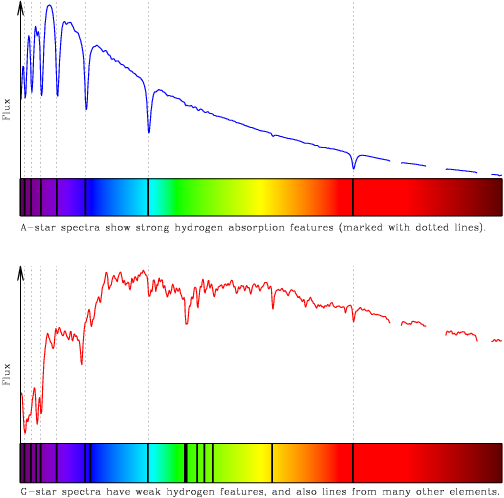
\includegraphics[width=0.9\textwidth,trim={0cm 9.75cm 0cm 0cm},clip]{Images/spectrum.png}
        \caption{The spectrum of a star.}
        \label{fig:stellar_spec}
    \end{subfigure}
    \hfill
    \begin{subfigure}[b]{0.75\textwidth}
        \centering
        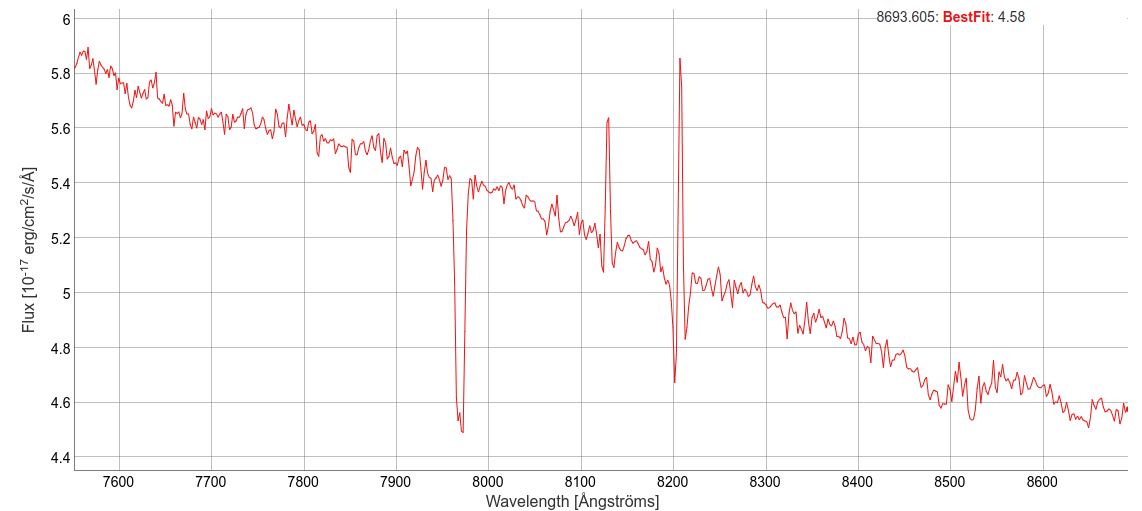
\includegraphics[width=0.9\textwidth,trim={0cm 0cm 0cm 1cm},clip]{Images/gal_spec.png}
        \caption{The spectrum of a galaxy.}
        \label{fig:gal_spec}
    \end{subfigure}
    \caption{}
    \label{fig:spec}
\end{figure}

\medskip
\textbf{Answer the following in your lab write-up}:
\begin{enumerate}
    \setcounter{enumi}{8}
    
    \item Describe some of the features (i.e., deviations from smoothness) that you see in the spectra in Figure \ref{fig:spec}.
    \item The color bar below Figure \ref{fig:stellar_spec} (the stellar spectrum) is an alternative representation of the spectrum. How do the features in the Flux vs. Wavelength plot correspond to the features on the color bar?
    \item What differences do you notice between the stellar spectrum and the galaxy spectrum? What are some similarities? Hypothesize as to \emph{why} the spectrum of a star differs from that of a galaxy.
\end{enumerate}

\subsection{Lamp Activity}
%H2, He, N, Ar, Hg, lightbulb

If you do not already have a \emph{diffraction grating}, come get one from me. A diffraction grating splits light into it's component colors, much like a prism. There are five lamps set up in the room; each lamp is actually heated gas of a specific element. Go up to each lamp and look at it through your diffraction grating.  
\bigskip 

\textbf{Make a table in your lab write-up with the element name in the first column and a description of what you observe in the second column.}  Once you have observed each of the lamps, \textbf{answer the following questions in your write-up}:
\begin{enumerate}
    \setcounter{enumi}{11}
    \item How are each of these spectra similar?
    \item How are they different?
    \item Craft a hypothesis as to \textit{why} the lamps look different from each other when viewed through a diffraction grating.
    \item Now look at one of the light bulbs (a source of white light) in the room with your diffraction grating. How is the spectrum of the light bulb different from the element lamps?
\end{enumerate}

\begin{figure}[h!]
    \centering
    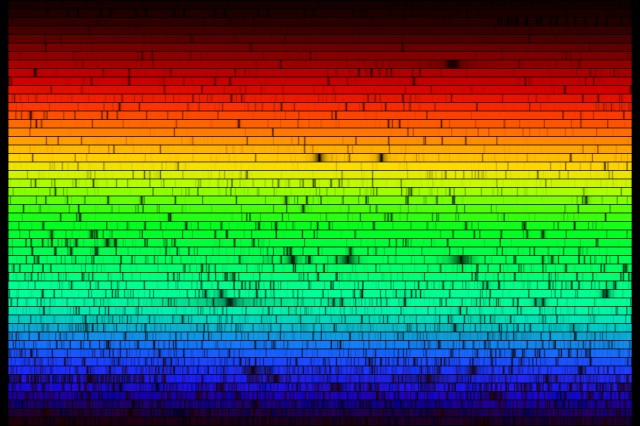
\includegraphics[width=0.7\textwidth]{Images/sun_spec.jpg}
    \caption{The spectrum of the Sun. Note that the actual spectrum should be one long, horizontal color gradient (like the ones seen through your diffraction gratings) -- this spectrum has been broken up into rows to fit onto the page and to show more detail.}
    \label{fig:sun}
\end{figure}

\noindent
Now check out Figure \ref{fig:sun}, the spectrum of the Sun. \textbf{Answer the following in your lab write-up}:
\begin{enumerate}
    \setcounter{enumi}{15}
    \item How is the Sun's spectrum different from the lamp spectra and the light bulb spectrum?
\end{enumerate}

\bigskip

Figure \ref{fig:types} shows three different types of spectra and how they're formed. Blackbodies emit across all wavelengths and thus have a \textbf{continuous spectrum}. A sample of gas is usually a conglomerate of multiple different chemical elements, so when the atoms of a gas are heated, they emit light at certain wavelengths, thus forming an \textbf{emission spectrum}. By contrast, if light from a blackbody or a continuous spectrum passes \emph{through} a gas, the atoms of the gas absorb some light, yielding an \textbf{absorption spectrum}. Due to the quantum nature of atoms, each element and molecule absorbs or emits at a unique set of wavelengths; each element has its own spectral ``fingerprint'' that can be used to uniquely identify the chemical makeup of an object.

\begin{figure}[h!]
    \centering
    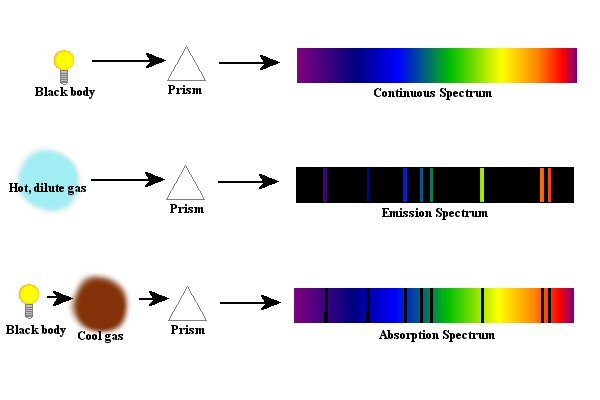
\includegraphics[width=0.9\textwidth,trim={0cm 2cm 0cm 1cm},clip]{Images/emission_v_absorption.jpg}
    \caption{Types of spectra.}
    \label{fig:types}
\end{figure}

\medskip 
\textbf{In your lab write-up, answer the following}, based on Figure \ref{fig:types}:
\begin{enumerate}
    \setcounter{enumi}{16}
    
    \item What type of spectrum matches the Sun's spectrum? Why do you think the Sun has this particular type of spectrum? (Hint: we observe light coming from the Sun's photosphere, but the Sun's corona lies between the photosphere and us)
    
    \item What type of spectrum matches the light bulb spectrum?
    
    \item What type of spectrum matches the lamp spectra?
\end{enumerate}


\subsection{Decomposing the Stars}
The spectral fingerprints we just explored allow astronomers to probe the chemical compositions of stars, galaxies, and planets. If we see an absorption line that we know is from carbon, then we know that there must be carbon in the star. The deeper the carbon absorption line in the spectrum, the more carbon there must be.

\medskip \noindent
You should each have two worksheets: one should have spectra for seven different elements and one should have spectra for three different stars. 

\textbf{In your lab write-up, complete the following}:
\begin{enumerate}
    \setcounter{enumi}{19}
    
    \item Make a table with a column for each element and a row for each star. Record which elements you find in each star by lining up the spectra of each element with the spectra of each star.
    
    \item Which elements are in every star?
    
\end{enumerate}
%\url{https://mrmacha.weebly.com/uploads/5/0/3/9/50390227/star_emission_spectrum_ws.pdf}


%%%%%%%%%%%%%%%%%%%%%%% REDSHIFT %%%%%%%%%%%%%%%%%%%%%%%
\section{Spectra and Motion: Oneshift, Twoshift, Redshift, Blueshift}
%Redshift and Blueshift

Spectra are not only useful for chemistry -- we can also use spectroscopy to study the \emph{motions} of astronomical bodies. Much like how the pitch of an ambulance changes as it moves towards or away from you, the wavelength of light changes depending on the motion of the light source -- this is a manifestation of the \emph{Doppler effect}. As a source of light moves towards you, the emitted light waves are \emph{compressed}, yielding shorter, bluer wavelengths: this is called \emph{blueshift}. Similarly, if a source of light is moving away from you, the light waves are \emph{stretched}, yielding longer, redder wavelengths: this is called \emph{redshift}. For fun, you can check out \url{https://javalab.org/en/doppler_effect_and_redshift_en/} to see blueshift and redshift in action. 

\begin{figure}[h!]
    \centering
    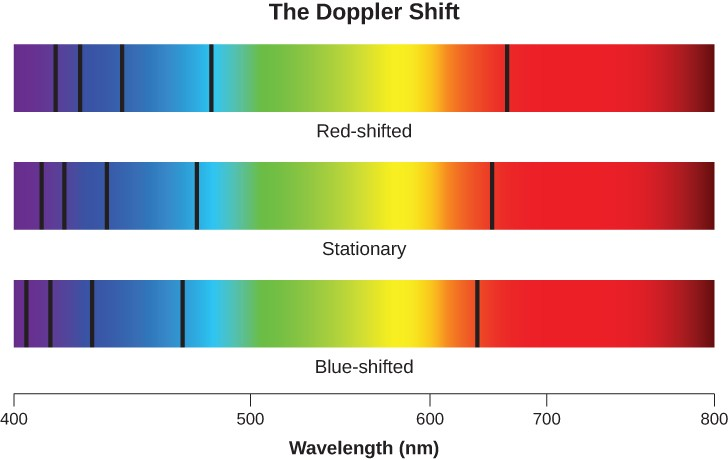
\includegraphics[width=0.75\textwidth]{Images/redshift.jpg}
    \caption{Redshift vs. Blueshift}
    \label{fig:redshift}
\end{figure}

\medskip \noindent
This redshift or blueshift manifests itself in the spectra of moving objects, as shown in Figure \ref{fig:redshift}. The middle row of Figure \ref{fig:redshift} shows the spectrum in the \emph{rest-frame} of the object -- that is, this is the spectrum we would observe if the object were perfectly stationary. \textbf{Answer the following in your lab write-up}:

\begin{enumerate}
    \setcounter{enumi}{21}
    
    \item The spectrum on the top row of Figure \ref{fig:redshift} corresponds to an object moving \emph{away} from us. How do the positions of the spectral absorption lines differ from those in the stationary spectrum? Are these features shifted towards bluer or redder wavelengths?
    
    \item The spectrum on the bottom row of Figure \ref{fig:redshift} corresponds to an object moving \emph{towards} us. How do the positions of the spectral absorption lines differ from those in the stationary spectrum? Are these features shifted towards bluer or redder wavelengths?
    
    \item Because the Universe is expanding, most objects are moving \emph{away} from us. Consider a galaxy moving with the expansion of the Universe: how would the galactic spectrum we \emph{observe} differ from the spectrum in the rest-frame of the galaxy? 
\end{enumerate}


\medskip
We can quantify the shift in a spectrum via the quantity $z$, often just referred to as \emph{the} redshift (even though it quantifies both blue-shifts and red-shifts). If an object at rest emits light of wavelength $\lambda_{\rm rest}$, but we observe that light at a redder or bluer wavelength, $\lambda_{\rm obs}$, due to the motion of the object, then the redshift, $z$, of the object is given by
\begin{equation} \label{eq:redshift}
    z = \frac{\lambda_{\rm obs}-\lambda_{\rm rest}}{\lambda_{\rm rest}}
\end{equation}
\noindent


\section{Wrapping things up}
\textbf{In your lab write-up, reflect on the following}:
\begin{enumerate}
    \setcounter{enumi}{24}
    
    \item Qualitatively describe what the \emph{spectrum} of an object is.
    
    \item What can we learn by studying the spectra of astronomical objects (i.e., what information does \emph{spectroscopy} give us)?
    
    \item Look back on what you've learned in lab so far and describe three different ways astronomers use light to learn about the Universe.
    
    \item \emph{Hubble's law} states that, on sufficiently large scales, objects that are \emph{further} away from us are moving away from us \emph{more quickly}. What does Hubble's Law imply about the relationship between redshift and an object's distance from us? (We'll talk much more about Hubble's law in a later lab.)
    
    \item How do you think one could use spectroscopy to determine the rotation speed of a star? (Hint: You can take individual spectra of different parts of the star. You should also think about how the material on the surface of the star is moving relative to the observer)
    
    \item Write down at least one question that you still have after finishing this lab.
    
    \item If you have any feedback on how today's lab was run, or if you have any suggestions for future lab sessions, please let me know!
    
\end{enumerate}

\end{document}
